Now that discrete components were analyzed, the impedance is expected to be accurate for the following tests. It is then possible to measure the impedance of a complex system: saline water. A solution of saline water at 22 $^{\circ}$C is passed in a 180 $\mu m$ wide PDMS microchannel in the microfluidic system presented in \autoref{sec:PracticalMicrofluidic}, and the impedance spectroscopy is measured the same way as was done in \autoref{sec:DiscreteResults}. The calibrated and converted impedance curves are obtained and shown in \autoref{fig:SalineImpedanceSine}. \par
\begin{figure}[h]
\centering
\begin{subfigure}{0.99\textwidth}
\centering
    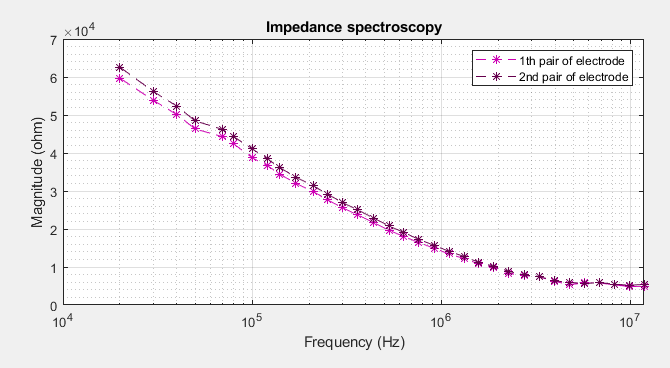
\includegraphics[width=0.9\linewidth]{SalineMagnitudeSine2}
    \caption{Magnitude.}
    \label{fig:SalineSineMagnitude2}
\end{subfigure}
\begin{subfigure}{0.99\textwidth}
\centering
    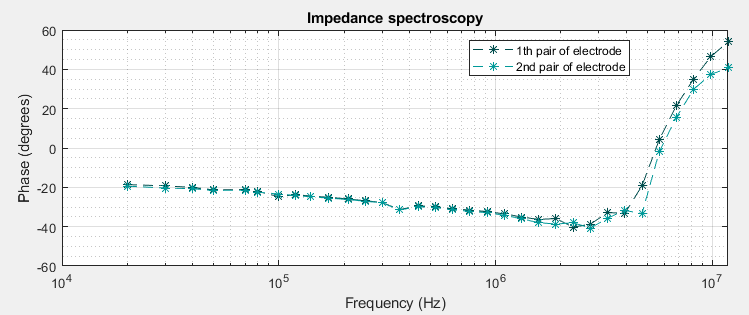
\includegraphics[width=0.9\linewidth]{SalinePhaseSine2}
    \caption{Phase.}
    \label{fig:SalinePhaseSine2}
\end{subfigure}
\caption{Bode plot of the calibrated impedance of a saline solution at 22 $^{\circ}$C containing 15g of salt for 100g of deionized water, after conversion from square to sine spectroscopy, measured by the two pairs of electrodes.}
\label{fig:SalineImpedanceSine}
\end{figure}

It is possible to see from \autoref{fig:SalineImpedanceSine} just how similar the responses of the two electrode pairs are. This proves the efficiency of the calibration step. The curves adequately represents some kind of a series capacitor and resistor, as was represented before in \autoref{fig:EIS_simplemodel}. 